\chapter{Übersicht der Hardware}
Wie auf diesem Schaltbild \rAbb{pic001} zu sehen ist, lässt sich die verwendete Hardware grob in drei Teilaspekte einteilen.
\begin{itemize}
	\item Aufnahme der Messdaten über die Sensoren
	\item Beschaltung und Wechsel zwischen den einzelnen Sensoren als Signalquelle
	\item AD-Wandlung und Seriellisierung der Daten mit abschießendem Senden an der Computer
\end{itemize}

\begin{figure}[h]
	\centering
	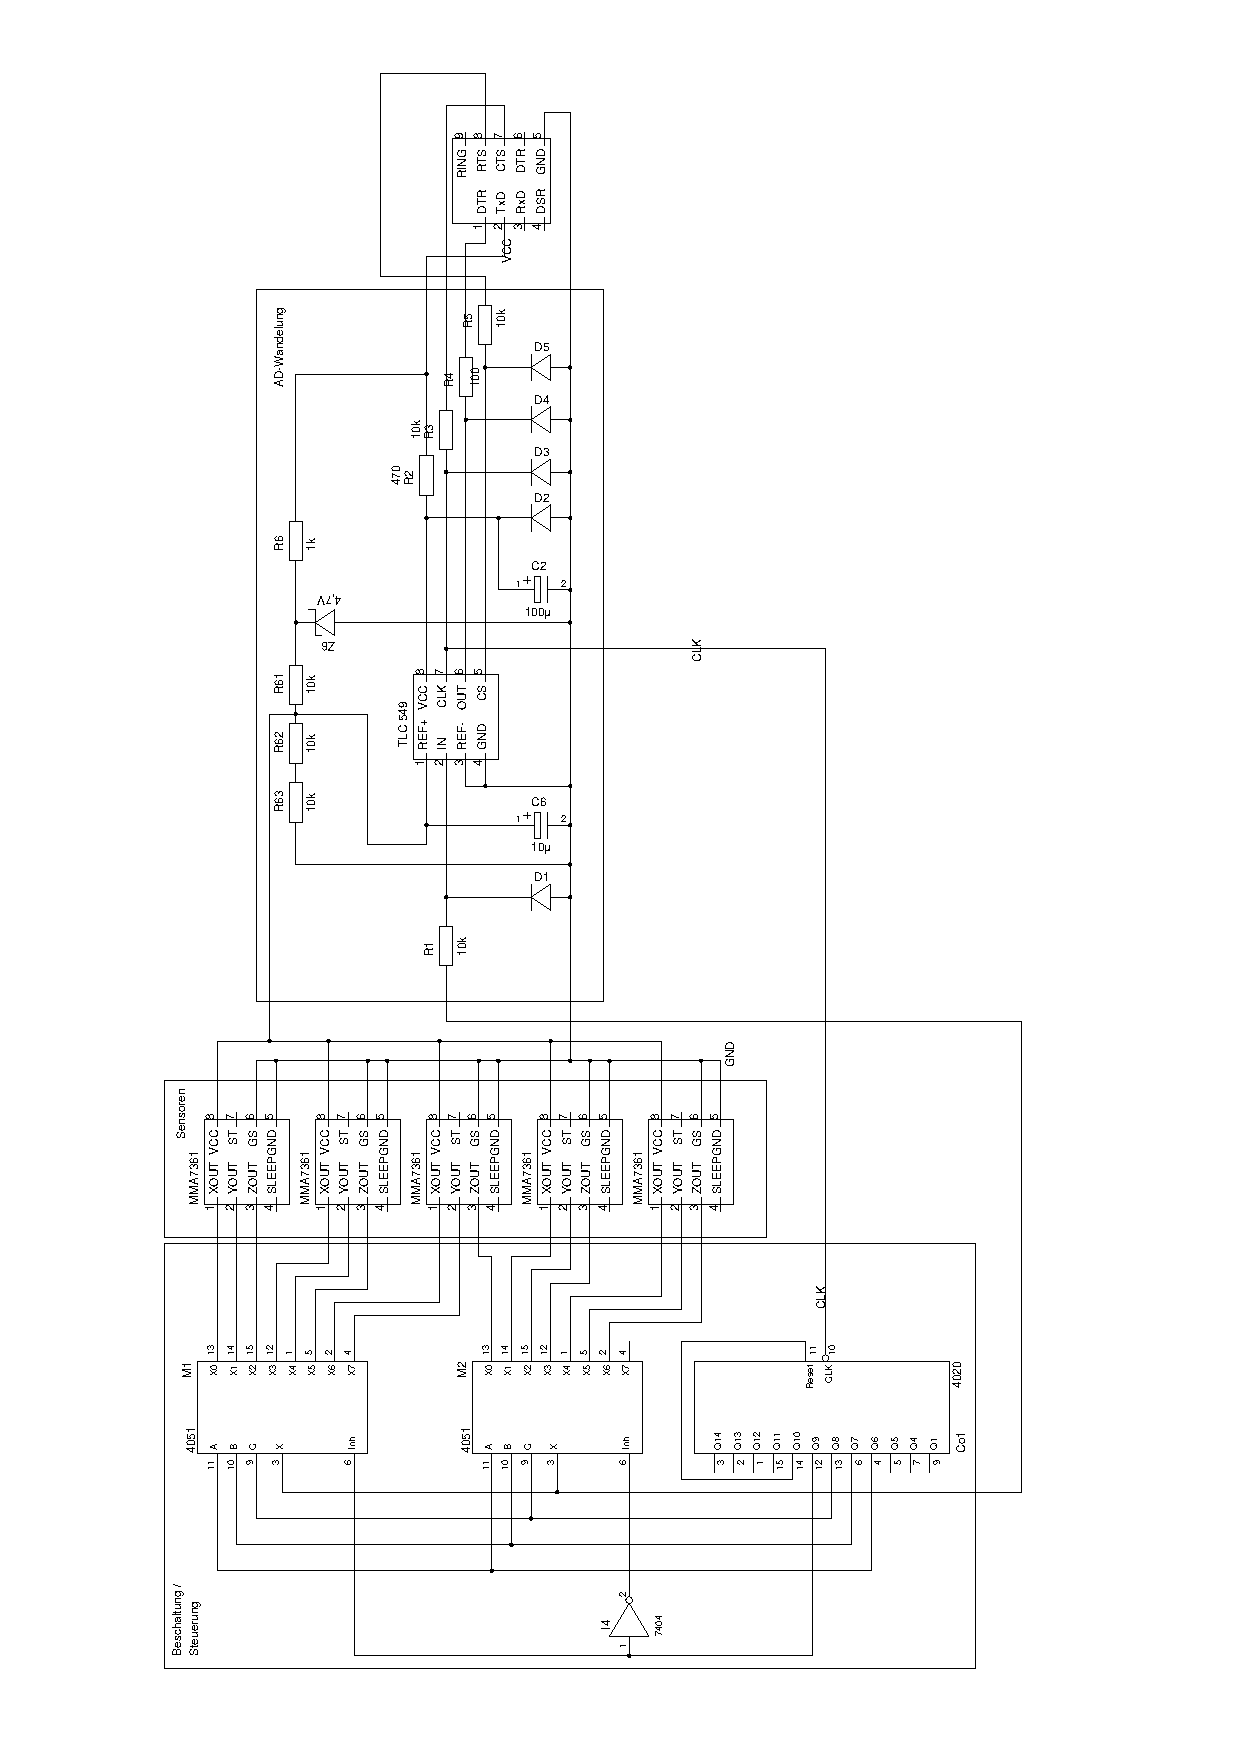
\includegraphics[scale=0.5]{pic/Mainpage.pdf}
	\caption{Gesamtschaltplan}
	\label{pic001}
\end{figure}

\chapter{Einzelne Teile der Hardware}
\section{Aufnahme der Messdaten}
Die Bewegung der Fingerkuppen wird über fünf Beschleunigungssensoren des Typs \partno{MMA7361LC} von Freescale Semiconductor aufgenommen. Dies sind kapazitive Beschleunigungssensoren mit einer Sensibilitätsspannweite bis 1.5g. Bei den genutzten Einstellungen beträgt die Sensitivität 800mV / g. Somit ist dieser Sensor nicht zuletzte aufgrund seines geringen Preises für die erste Testphase des Handschuhprojektes gut geeignet. Die Sensoren sind an \textbf{GND} und an eine spannungsführende Linie mit 3,13V angeschlossen. \partno{g-select} wird ebenfalls an \textbf{GND} angeschlossen, um die Sensitivitätsgrenze von 1.5g zu wählen.
Die Sensoren geben drei analoge Spannungssignale aus - eins für jede Achse. Die Höhe der Spannung gibt den aktuelle Beschleunigungswert an. Die insgesamt 15 Datenleitungen werden in den nächsten Abschnitt geführt.

\section{Beschaltung und Wechsel}
Durch die Wahl der Sensoren treffen 15 Datenleitungen gleichzeitig ein und sollen ausgelesen werden. Hier gibt es nun zwei Alternativen:
\begin{nListe}
\item Die Daten werden serialisiert und nacheinander an den auswertenden Computer gesendet
\item Die Daten werden parallel an den Computer gesendet
\end{nListe}
Die Nachteile der beiden Alternativen sind klar. Bei der seriellen Datensendung gehen bei geringen Übertragungsraten viele Daten verloren. Die paralelle Alternative ist zwar schneller, hat aber auch ihren Preis. Statt einem Eingang und einem AD-Wandler werden gleich 15 davon benötigt. Zu lösen ist dieses Problem über teure Laborkarten, die eigens für wissenschaftliche Zwecke hergestellt wurden. In diesem Projekt wird jedoch die erste Möglichkeit - serielle Datensendung - verwendet.
Deshalb wird mit einem 14-Ripple-Counter \partno{74HC 4020}, zwei analogen (De)Multiplexern \partno{74HC 4051} und einem Inverter gearbeitet. Das Prinzip ist folgendes: Der Counter erhält vom Computer ein Tick-Signal und erhöht den internen Speicher um eins. Daraus folgt eine Freischaltung eines bestimmten damit verknüpften Kanals der beiden Multiplexer. Der höchste benutzte Counterausgang steuert nun, welcher der beiden Multiplexer angesteuert wird. Hat der Counter alle Kanäle der Multiplexer einmal durchgeschalten, setzt er sich selbst auf Reset und das Intervall beginnt von vorne. Insgesamt werden somit 16 Kanäle angesteuert - von denen 15 belegt sind - und der Spannungswert jeweils an die Wandlung gesandt. Der Grund für das Auslassen der ersten drei Counterausgänge liegt in der Gesamtzeitsteuerung. In der Zeit, in der der Counter diese $2^3 = 8$ Schritte durchläuft wird das digitalisierte Signal an den Computer gesendet (siehe \rTab{pic002}). 
Multiplexer, Inverter und Counter sind jeweils an \textbf{GND} und \textbf{PWR} angeschlossen.

\section{AD-Wandler}
Durch die Beschaltung werden die 15 (eigentlich 16) Spannungswerte an den AD-Wandler gesendet. Dort werden sie digitalisiert auf 8 Bit und über die Datenleitung nacheinander an die serielle Schnittstelle gesendet. Der verwendete AD-Wanlder \partno{TLC548C} funktioniert nach der \textit{Sample-and-hold}-Technik. Dabei wird vom Computer ein Signal (\textbf{CS}) zum Speichern des Messwertes gegeben. 17$\mu$s danach steht der digitale Wert am Ausgang bereit und kann durch Setzten und Löschen des Clockeingangs abgerufen werden. Aus diese Weise ist er schon serialisiert und wird in diesem Rohformat über die serielle Datenleitung gesendet. Wohlgemerkt handelt es sich dabei nicht um Datenpakete nach einem bestimmten Standard der serielle Datenleitung (siehe \rTab{pic003}). 

\begin{table}
	\centering
	\begin{tabular}{ccc}
		Counter & Offener Kanal des Multiplexers & Angezeigtes Bit des AD-Wandlers \\ \hline
		0&0&8 (von Ch.16)\\
		1&0&7 (von Ch.16)\\
		2&0&6 (von Ch.16)\\
		3&0&5 (von Ch.16)\\
		4&0&4 (von Ch.16)\\
		5&0&3 (von Ch.16)\\
		6&0&2 (von Ch.16)\\
		7&0&1 (von Ch.16)\\
		&&CS-Select ausführen\\
		8&1&8 (von Ch.1)\\
		9&1&7 (von Ch.1)\\
		10&1&6 (von Ch.1)\\
		11&1&5 (von Ch.1)\\
		12&1&4 (von Ch.1)\\
		13&1&3 (von Ch.1)\\
		14&1&2 (von Ch.1)\\
		15&1&1 (von Ch.1)\\
		\dots&&\\
		65&9&8 (ab hier wird der zweite Multiplexer aktiviert)
		
	\end{tabular}
	\caption{Zeitlicher Verlauf der einzelnen Steursignale}
	\label{pic002}
\end{table}

\begin{table}[t]
	\centering
	\begin{tabular}{lccccccc}
	ca 17 $\mu$s & ca 2 $\mu$s & ca 2 $\mu$s &ca 2 $\mu$s &ca 2 $\mu$s &ca 2 $\mu$s &ca 2 $\mu$s &ca 2 $\mu$s &ca 2 $\mu$s &\\
	
	\end{tabular}
	\caption{Zeitlicher Verlauf der Daten auf der Datenleitung der seriellen Verbindung}
	\label{pic003}
\end{table}